%  links for CASE 2016, http://case2016.org/  
% https://ras.papercept.net/conferences/scripts/login.pl      to submit
% https://ras.papercept.net/conferences/scripts/pdftest.pl  to test pdf

% obstacles: brown
% robots: blue

%(Note:   Similar games are SuperFruitfall and Denki Blocks). 


\documentclass[letterpaper, 10 pt, conference]{ieeeconf}
\IEEEoverridecommandlockouts
%\documentclass[12pt]{article}
%\usepackage{times}
\usepackage{calc}
\usepackage{url}
\usepackage{hyperref}
\hypersetup{
  colorlinks =true,
  urlcolor = black,
  linkcolor = black
}
\usepackage{graphicx}
\usepackage[cmex10]{amsmath}
\usepackage{bm}
\usepackage{amssymb}
\usepackage{rotating}


%\usepackage{xfrac}
\usepackage{nicefrac}
\usepackage{cite}
\usepackage[caption=false,font=footnotesize]{subfig}
\usepackage[usenames, dvipsnames]{color}
\usepackage{colortbl}
%\usepackage{caption}

%\usepackage{wrapfig}
\usepackage{overpic}
%\usepackage{subfigure}
%\usepackage{textcomp}
\graphicspath{{./pictures/pdf/},{./pictures/ps/},{./pictures/png/},{./pictures/jpg/},{./code/Data/}}
\usepackage{breqn} %for breaking equations automatically
\usepackage[ruled]{algorithm}
\usepackage{algpseudocode}
%\usepackage{algorithmic}
\usepackage{multirow}
\usepackage{todonotes}

%\newcommand{\todo}[1]{\vspace{5 mm}\par \noindent \framebox{\begin{minipage}[c]{0.98 \columnwidth} \ttfamily\flushleft \textcolor{red}{#1}\end{minipage}}\vspace{5 mm}\par}
% uncomment this to hide all red todos
%\renewcommand{\todo}{}

%% ABBREVIATIONS
\newcommand{\qstart}{q_{\text{start}}}
\newcommand{\qgoal}{q_{\text{goal}}}
\newcommand{\pstart}{p_{\text{start}}}
\newcommand{\pgoal}{p_{\text{goal}}}
\newcommand{\xstart}{x_{\text{start}}}
\newcommand{\xgoal}{x_{\text{goal}}}
\newcommand{\ystart}{y_{\text{start}}}
\newcommand{\ygoal}{y_{\text{goal}}}
\newcommand{\gammastart}{\gamma_{\text{start}}}
\newcommand{\gammagoal}{\gamma_{\text{goal}}}
\providecommand{\proc}[1]{\textsc{#1}}


\newcommand{\ARLfull}{Aero\-space Ro\-bot\-ics La\-bora\-tory }
\newcommand{\ARL}{\textsc{arl}}
\newcommand{\JPL}{\textsc{jpl}}
\newcommand{\PRM}{\textsc{prm}}

\newcommand{\CM}{\textsc{cm}}
\newcommand{\SVM}{\textsc{svm}}
\newcommand{\NN}{\textsc{nn}}
\newcommand{\prm}{\textsc{prm}}
\newcommand{\lemur}{\textsc{lemur}}
\newcommand{\Lemur}{\textsc{Lemur}}
\newcommand{\LP}{\textsc{lp}} 
\newcommand{\SOCP}{\textsc{socp}}
\newcommand{\SDP}{\textsc{sdp}}
\newcommand{\NP}{\textsc{np}}
\newcommand{\SAT}{\textsc{sat}}
\newcommand{\LMI}{\textsc{lmi}}
\newcommand{\hrp}{\textsc{hrp\nobreakdash-2}}
\newcommand{\DOF}{\textsc{dof}}
\newcommand{\UIUC}{\textsc{uiuc}}
%% MACROS


\providecommand{\abs}[1]{\left\lvert#1\right\rvert}
\providecommand{\norm}[1]{\left\lVert#1\right\rVert}
\providecommand{\normn}[2]{\left\lVert#1\right\rVert_#2}
\providecommand{\dualnorm}[1]{\norm{#1}_\ast}
\providecommand{\dualnormn}[2]{\norm{#1}_{#2\ast}}
\providecommand{\set}[1]{\lbrace\,#1\,\rbrace}
\providecommand{\cset}[2]{\lbrace\,{#1}\nobreak\mid\nobreak{#2}\,\rbrace}
\providecommand{\lscal}{<}
\providecommand{\gscal}{>}
\providecommand{\lvect}{\prec}
\providecommand{\gvect}{\succ}
\providecommand{\leqscal}{\leq}
\providecommand{\geqscal}{\geq}
\providecommand{\leqvect}{\preceq}
\providecommand{\geqvect}{\succeq}
\providecommand{\onevect}{\mathbf{1}}
\providecommand{\zerovect}{\mathbf{0}}
\providecommand{\field}[1]{\mathbb{#1}}
\providecommand{\C}{\field{C}}
\providecommand{\R}{\field{R}}
\newcommand{\Cspace}{\mathcal{Q}}
\newcommand{\Uspace}{\mathcal{U}}
\providecommand{\Fspace}{\Cspace_\text{free}}
\providecommand{\Hcal}{$\mathcal{H}$}
\providecommand{\Vcal}{$\mathcal{V}$}
\DeclareMathOperator{\conv}{conv}
\DeclareMathOperator{\cone}{cone}
\DeclareMathOperator{\homog}{homog}
\DeclareMathOperator{\domain}{dom}
\DeclareMathOperator{\range}{range}
\DeclareMathOperator{\sign}{sgn}
\providecommand{\polar}{\triangle}
\providecommand{\ainner}{\underline{a}}
\providecommand{\aouter}{\overline{a}}
\providecommand{\binner}{\underline{b}}
\providecommand{\bouter}{\overline{b}}
\newcommand{\D}{\nobreakdash-\textsc{d}}
%\newcommand{\Fspace}{\mathcal{F}}
\providecommand{\Fspace}{\Cspace_\text{free}}
\providecommand{\free}{\text{\{}\mathsf{free}\text{\}}}
\providecommand{\iff}{\Leftrightarrow}
\providecommand{\subinner}[1]{#1_{\text{inner}}}
\providecommand{\subouter}[1]{#1_{\text{outer}}}
\providecommand{\Ppoly}{\mathcal{X}}
\providecommand{\Pproj}{\mathcal{Y}}
\providecommand{\Pinner}{\subinner{\Pproj}}
\providecommand{\Pouter}{\subouter{\Pproj}}
\DeclareMathOperator{\argmax}{arg\,max}
\providecommand{\Aineq}{B}
\providecommand{\Aeq}{A}
\providecommand{\bineq}{u}
\providecommand{\beq}{t}
\DeclareMathOperator{\area}{area}
\newcommand{\contact}[1]{\Cspace_{#1}}
\newcommand{\feasible}[1]{\Fspace_{#1}}
\newcommand{\dd}{\; \mathrm{d}}
\newcommand{\figwid}{0.22\columnwidth}
\newcommand{\TRUE}{\textbf{true}}
\newcommand{\FALSE}{\textbf{false}}
\DeclareMathOperator{\atan2}{atan2}


\newtheorem{theorem}{Theorem}
\newtheorem{definition}[theorem]{Definition}
\newtheorem{lemma}[theorem]{Lemma}
\begin{document}

%%%%%%%%%%%%%% For debugging purposes, I like to display the TOC
%    \tableofcontents
%    \setcounter{tocdepth}{3}
%\newpage
%\mbox{}
%\newpage
%\mbox{}
%\newpage

%%%%%% END TOC %%%%%%%%%%%%%%%%%%%%%%%%%%%%%%%%%%%%%%%

\title{\LARGE \bf 
Object Manipulation and Position Control \\Using a Swarm With Global Inputs
%Force and Torque Control using a Swarm With Global Inputs
}
\author{Shiva Shahrokhi and  Aaron T. Becker%, 
\thanks{{S. Shahrokhi and A. Becker are with the Department of Electrical and Computer Engineering,  University of Houston, Houston, TX 77204-4005 USA {\tt\small  \{sshahrokhi2, atbecker\}@uh.edu}
}
} %\end thanks
} % end author block
\maketitle

\begin{abstract}
Manipulating objects with a swarm of simple robots with global control inputs is difficult because they are highly under-actuated, the number of robots in contact with object changes dynamically, the robots contacting each other changes dynamically, and because the robots disperse over time they must be recollected.

Micro and nano robots are suited for targeted drug delivery and micro scale manufacturing because they are small enough to navigate the passageways of the body. 
However, due to their small size, micro robots cannot contain onboard processing for autonomy nor onboard power. 
Instead they are controlled by an external signal such as a magnetic field. 
Because each robot can only provide a small amount of force or transport a small amount of material, large swarms of robots are required, all controlled by the same external field. 

This work presents controllers and algorithms for steering such an under-actuated swarm to manipulate objects. 
Previous work showed that mean and variance of the swarm is controllable. 
This was used to manipulate convex polygonal objects through a simple maze. 
A key remaining challenge is controlling the torque applied to an object. 
Torque control is necessary for manipulating objects as well as for aligning sensors, emitters, or redirecting an incoming signal.
This work first proves that swarm torque control is possible, then presents algorithms to automate the task. 
The paper concludes with experimental results using 97 hardware robots to manipulate rectangles with large aspect ratios.

%
%Micro- and nano-robots can be manufactured in large numbers. Large numbers of micro robots are required in order to deliver sufficient payloads, but the small size of these robots makes it difficult to perform onboard computation.  Instead, these robots are often controlled by a global, broadcast signal. 
%In our previous work we focused on a block-pushing task, where a swarm of robots pushed a larger block through a 2D maze. One surprising result was that humans that only knew the swarm's mean and covariance completed the task faster that humans who knew the position of every robot~\cite{Becker2013b}. 
%Inspired by that work, we proved that we can control the mean position of a swarm and that with an obstacle we can control the swarm's position variance ($\sigma_x$ and $\sigma_y$). 
%We then wrote automatic controllers which could complete a block pushing task, but these controllers had some limitations~\cite{ShahrokhiIROS2015}. 
%One of the limitations was that we could only compress our swarm along the world $x$ and $y$ axes, and could not navigate workspaces with narrow corridors with other orientations. 
%One solution to these problems would be a controller that regulates the swarm's position covariance, $\sigma_{xy}$. 
%For controlling $\sigma_{xy}$, we prove that the swarm position covariance $\sigma_{xy}$ is controllable given boundaries with non-zero friction. 
%We then prove that two orthogonal boundaries with high friction are sufficient to arbitrarily position a swarm of robots. 
%We conclude by designing controllers that efficiently regulate $\sigma_{xy}$.
\end{abstract}

%TODO: new outline

%%%%%%%%%%% PAPER OUTLINE
% INTRODUCTION, Related work
%      micro/nano applications
%	open questions in swarm control
% 	difficulties in obtaining experimental data
% Theory:
%% Wall friction shape
%% Control 2 robots
% Simulation:
%% Use wall friction to control covariance 1. Make variances small(feedback), 2. Move Swarm to wall, 3. drag out swarm to achieve covariance(feedback) 4. Move to goal.
%% Algorithm to control position of 2 robots using friction
%%%%%%% Algorithm to control position of n robots using friction
% Experiment
%% Use wall friction to control covariance
%% Algorithm to control position of 2 robots using friction
%%Future Work

%%%%%%%%%%%%%%%
%\todo{image 1 should be the kilobots pushing an interesting object.  Current images 1 and 2 are not attractive, have the same caption, and the robots look like ellipses}
\section{Introduction}\label{sec:Intro}
%This project studies system models and user interfaces for five multi-robot manipulation tasks with large populations of micro- and nanorobots.  We test several system models with different limitations on controllability and observability of the motion controller, and evaluate several different user interfaces.  We conduct user experiments to understand the impact of these limitations and design choices. 


%Micro- and nanorobotics have the potential to revolutionize many applications including targeted material delivery, assembly, and surgery.  The same properties that promise breakthrough solutions---small size and large populations---present unique challenges to generating controlled motion.  
Large populations of micro- and nanorobots are being produced in laboratories around the world, with diverse potential applications in drug delivery and construction \cite{Peyer2013,Shirai2005,Chiang2011}. These activities require robots that behave intelligently.
Limited computation and communication rules out autonomous operation or direct control over individual units; instead we must rely on global control signals broadcast to the entire robot population.  It is not always practical to gather pose information on individual robots for feedback control; the robots might be difficult or impossible to sense individually due to their size and location. However, it is often possible to sense global properties of the group, such as mean position and density.  Finally, many promising applications will require direct human control, but user interfaces to thousands---or millions---of robots is a daunting human-swarm interaction (HSI) challenge. 

Our previous work with over a hundred hardware robots and thousands of simulated robots~\cite{Becker2013b} demonstrated that direct human control of large swarms is possible. Unfortunately, the logistical challenges of repeated experiments with over one hundred robots prevented large-scale tests. To gather better data, we designed a large-scale online game to test how humans interact with large swarms.  These  experiments~\cite{Becker2014e} showed that numerous simple robots responding to global control inputs are directly controllable by a human operator without special training, and that the visual feedback of the swarm state should be very simple in order to increase task performance.


\begin{figure}
\centering
\begin{overpic}[width=\columnwidth *4 /5]{BlockPushing.png}\end{overpic}
\todo{I like the 'target' symbol, but it is not self-documenting.  We need a legend explaining the min and max variance ellipses, the goal region, the variance, the mean, the object COM, and the target mean position.  I think these are easiest to make in powerpoint.
Please use the same color and line style for the variance min and max as you use in Figure 4.
}
%{blockpushingImageWithMeanAndVarianceOverlay.png}
\caption{\label{fig:bigPictureMeanAndVarianceForSwarm} A swarm of robots, all controlled by the same, uniform force field, can be effectively controlled hybrid controller that knows only the first and second moments of the robot distribution.  Here a swarm of simple robots (blue discs) pushes a green block toward the goal.}
\end{figure}


%\begin{figure}
%\renewcommand{\figwid}{0.32\columnwidth}
%\subfloat[][Vary Number]{\label{fig:VaryNum}
%\begin{overpic}[width =\figwid]{VaryNum.pdf}\end{overpic}}
%%
%\subfloat[][Vary Visual Feedback]{\label{fig:VaryVis}
%\begin{overpic}[width =\figwid]{VaryVisFS.pdf}\end{overpic}
%\begin{overpic}[width =\figwid]{VaryVisMV.pdf}\end{overpic}}\\
%%
%\subfloat[][Vary Control]{\label{fig:VaryControl}
%\begin{overpic}[width =\figwid]{VaryControl.pdf}\end{overpic}}
%%
%\subfloat[][Vary Noise]{\label{fig:VaryNoise}
%\begin{overpic}[width =\figwid]{VaryNoise.pdf}\end{overpic}}
%%
%\subfloat[][Control Position]{\label{fig:ControlPos}
%\begin{overpic}[width =\figwid]{ControlPos.pdf}\end{overpic}}
%%
%\caption{\label{fig:5experiments}
%Screenshots from our five online experiments controlling multi-robot systems with limited, global control.
%\textbf{(a)} Varying the number of robots from 1-500
%\textbf{(b)} Comparing 4 levels of visual feedback 
%\textbf{(c)} Comparing 3 control architectures
%\textbf{(d)} Varying noise from 0 to 200\% of control authority
%\textbf{(e)} Controlling the position of 1 to 10 robots.
%\href{http://youtu.be/HgNENj3hvEg}{See video overview at http://youtu.be/HgNENj3hvEg.}
%\vspace{-2em}
%}
%\end{figure}






% Our paper is organized as follows.  After a discussion of related work in Section \ref{sec:RelatedWork}, we describe our experimental methods for an online human-user experiment in Section \ref{sec:expMethods}.  We report the results of our experiments in Section \ref{sec:expResults}, discuss the lessons learned in Section \ref{sec:discussion}, and end with concluding remarks in Section \ref{sec:conclusion}.



%%%%%%%%%%%%%%%
\section{Related Work}
\label{sec:relatedWork}



\subsection{How to control mean}

In our previous work, we proved that we can easily control mean position of the swarm. We control mean position with a PD controller that uses the mean position and mean velocity. Our control input is the global force applied to each robot:
\begin{align}
u_x &= K_{p}(x_{goal} - \bar{x}) + K_{d}(0-\bar{v}_x) \nonumber\\
u_y &= K_{p}(y_{goal}  - \bar{y}) + K_{d}(0-\bar{v}_y)  \label{eq:PDcontrolPosition}
\end{align}
here $K_{p}$ is the proportional gain, and $K_{d}$ is the derivative gain. We performed a parameter sweep to identify the best values.  Representative experiments are shown in Fig.~\ref{fig:gainvalues}. 100 robots were used and the maximum speed was 3 meters per second. As shown in Fig.~\ref{fig:gainvalues}, we can achieve an overshoot of 1\% and a  rise time of 1.52 s with $K_{p}= 4$, and  $K_{d} = 1$. 

\begin{figure}
\centering
\begin{overpic}[width = \columnwidth]{gainvalues.eps}
\end{overpic}
\vspace{-1em}
\caption{\label{fig:gainvalues} Tuning proportional ($K_p$, top) and derivative ($K_d$, bottom)  gain values in \eqref{eq:PDcontrolPosition} improves performance. These plots show convergence with 100 robots.
%\vspace{-2em}
}
\end{figure}

\subsection{How to control variance}

\begin{figure}
\centering
\begin{overpic}[width = \columnwidth] {brownianfig.eps}
\end{overpic}
\vspace{-1em}
\caption{\label{fig:varyBrownian} Increased noise results in more responsive variance control because stronger Brownian noise causes a faster increase of variance.
%\vspace{-2em}
}
\end{figure}

For variance control we move away from the wall and wait to increase variance because Brownian noise naturally disperses the swarm in such a way that the variance increases linearly.  If faster dispersion is needed, the swarm can be pushed through obstacles such as a diffraction grating or Pachinko board. %no need to worry about blocks in this controller.

The variance control law to regulate the variance to $\sigma^2_{ref}$ has three gains:
\begin{align}
u_x &= K_{p}(x_{goal}(\sigma^2_{ref}) - \bar{x}) - K_{d}\bar{v}_x + K_{i}(\sigma^2_{ref}-\sigma^2_{x}) \nonumber\\
u_y &= K_{p}(y_{goal}(\sigma^2_{ref})  - \bar{y}) - K_{d}\bar{v}_y + K_{i}(\sigma^2_{ref}-\sigma^2_{y}).  \label{eq:PDcontrolVariance}
\end{align}
In a slight abuse of notation we call the gain scaling the variance error $K_i$ because the variance integrates over time.
Eq.~\ref{eq:PDcontrolVariance} assumes the nearest wall is to the left of the robot at $x=0$, and chooses a reference goal position that in steady-state would have the correct variance:
\begin{align}
x_{goal}(\sigma^2_{ref}) = r + \sqrt{3\sigma^2_{ref}}
\end{align}
 If another wall is closer, the signs of $[K_p,K_i]$ are inverted, and the location $x_{goal}$ is translated.  Results are shown in Fig.~\ref{fig:varyBrownian}, with $K_{p,i,d} = [4,1,1]$.


%%%%%%%%%%%%%%%
%%%%%%%%%%%%%%%%%%%%%%%%%%%%%%%%%%%%%%%%%%%%%%%%%%%%%%%%%%%
\section{Theory}
\label{sec:theory}
%%%%%%%%%%%%%%%%%%%%%%%%%%%%%%%%%%%%%%%%%%%%%%%%%%%%%%%%%%%

\begin{algorithm}
\caption{GenerateDesired$x$-spacing($s_1,s_2,e_1,e_2,L$)}\label{alg:XControl}
\begin{algorithmic}[1]
\Require Knowledge of starting $(s_1,s_2)$ and ending $(e_1,e_2)$ positions of  two robots. 
$(0,0)$ is bottom corner, $s_1$ is topmost robot, 
 $L$ is length of the walls. Current position of the robots are $(r_1,r_2)$.
\Ensure   $ r_{1y} - r_{2y}  \equiv s_{1y} - s_{2y} $   %$\Delta y(t) \equiv \Delta y(0)$ 
\State $ \Delta s_x  \gets s_{1x} - s_{2x} $
\State $ \Delta e_x \gets e_{1x} - e_{2x} $
\State $ r_1 \gets s_1$, $ r_2 \gets s_2$
\If {$\Delta e_x < 0 $ }
\State $ m \gets ( L-\max( r_{1x},r_{2x}) ,0)   $ \Comment{Move to right wall}
\Else 
\State  $ m \gets ( -\min( r_{1x},r_{2x}),0 )    $ \Comment{Move to left wall}
\EndIf
\State $m  \gets  m + (0, -\min( r_{1y},r_{2y} ))$ \Comment{Move to bottom}
\State $ r_1 \gets r_1+m$, $ r_2 \gets r_2+m$ \Comment{Apply move}
\If {$\Delta e_x - (r_{1x} - r_{2x} ) > 0 $}
\State $ m \gets (\min(\|\Delta e_x - \Delta s_x \|, L- r_{1x}), 0)$  \Comment{Move right}
\Else
\State $ m \gets (-\min(\|\Delta e_x - \Delta s_x \|, r_{1x}), 0)$\Comment{Move left}
\EndIf 
\State $m  \gets  m + (0, \epsilon)$ \Comment{Move up}
\State $ r_1 \gets r_1+m$, $ r_2 \gets r_2+m$ \Comment{Apply move}
\State $\Delta r_x = r_{1x} - r_{2x}$
\If {$\Delta r_x \equiv \Delta e_x$} 
\State   $ m \gets (e_{1x}-r_{1x}, e_{1y}-r_{1y})$
\State $ r_1 \gets r_1+m$, $ r_2 \gets r_2+m$ \Comment{Apply move}
\State  \Return $(r_1,r_2)$
\Else   
\State \Return GenerateDesired$x$-spacing($r_1,r_2,e_1,e_2,L$)
\EndIf
\end{algorithmic}
\end{algorithm}

\begin{algorithm}
\caption{GenerateDesired$y$-spacing($s_1,s_2,e_1,e_2,L$)}\label{alg:YControl}
\begin{algorithmic}[1]
\Require Knowledge of starting $(s_1,s_2)$ and ending $(e_1,e_2)$ positions of  two robots. 
$(0,0)$ is bottom corner, $s_1$ is rightmost robot, 
 $L$ is length of the walls. Current position of the robots are $(r_1,r_2)$.
\Ensure   $ r_{1x} - r_{2x}  \equiv s_{1x} - s_{2x} $   %$\Delta y(t) \equiv \Delta y(0)$ 
\State $ \Delta s_y  \gets s_{1y} - s_{2y} $
\State $ \Delta e_y \gets e_{1y} - e_{2y} $
\State $ r_1 \gets s_1$, $ r_2 \gets s_2$
\If {$\Delta e_y < 0 $ }
\State $ m \gets ( L-\max( r_{1y},r_{2y}) ,0)   $ \Comment{Move to top wall}
\Else 
\State  $ m \gets ( -\min( r_{1y},r_{2y}),0 )    $ \Comment{Move to bottom wall}
\EndIf
\State $m  \gets  m + (0, -\min( r_{1x},r_{2x} ))$ \Comment{Move to left}
\State $ r_1 \gets r_1+m$, $ r_2 \gets r_2+m$ \Comment{Apply move}
\If {$\Delta e_y - (r_{1y} - r_{2y} ) > 0 $}
\State $ m \gets (\min(\|\Delta e_y - \Delta s_y \|, L- r_{1y}), 0)$  \Comment{Move top}
\Else
\State $ m \gets (-\min(\|\Delta e_y - \Delta s_y \|, r_{1y}), 0)$\Comment{Move bottom}
\EndIf 
\State $m  \gets  m + (0, \epsilon)$ \Comment{Move right}
\State $ r_1 \gets r_1+m$, $ r_2 \gets r_2+m$ \Comment{Apply move}
\State $\Delta r_y = r_{1y} - r_{2y}$
\If {$\Delta r_y \equiv \Delta e_y$} 
\State   $ m \gets (e_{1x}-r_{1x}, e_{1y}-r_{1y})$
\State $ r_1 \gets r_1+m$, $ r_2 \gets r_2+m$ \Comment{Apply move}
\State  \Return $(r_1,r_2)$
\Else   
\State \Return GenerateDesired$y$-spacing($r_1,r_2,e_1,e_2,L$)
\EndIf
\end{algorithmic}
\end{algorithm}

\begin{algorithm}
\caption{WallFrictionArrange2Robots($s_1,s_2,e_1,e_2,L$)}\label{alg:PosControl2Robots}
\begin{algorithmic}[1]
\Require 
Knowledge of starting $(s_1,s_2)$ and ending $(e_1,e_2)$ positions of  two robots. 
$(0,0)$ is bottom corner, $s_1$ is rightmost robot, 
 $L$ is length of the walls. 
 Current position of the robots are $(r_1,r_2)$.
\State $\Delta s_x \gets s_{1x} - s_{2x}$
\State $\Delta s_y \gets s_{1y} - s_{2y}$
\State $\Delta e_x \gets  e_{1x} - e_{2x} $
\State $ \Delta e_y \gets e_{1y} - e_{2y}$
\If {$\Delta s_x < \Delta s_y$}
\State GenerateDesired$x$-spacing($s_1,s_2,e_1,e_2,L$)
\State GenerateDesired$y$-spacing($s_1,s_2,e_1,e_2,L$)
\Else
\State GenerateDesired$y$-spacing($s_1,s_2,e_1,e_2,L$)
\State GenerateDesired$x$-spacing($s_1,s_2,e_1,e_2,L$)
\EndIf

\end{algorithmic}
\end{algorithm}


\begin{figure}
\centering
\begin{overpic}[width = \columnwidth]{Covariance.png}\end{overpic}
\vspace{-1em}
\caption{\label{fig:covFriction} We can control covariance of the swarm by using friction.
}\vspace{-1em}
\end{figure}


\section{Position Control of $n$ robots using wall friction}
Algorithm \ref{alg:PosControl2Robots}  can be extended to control the position of $n$ robots using wall friction under several constraints. Assume an open workspace with four axis-aligned walls with infinite friction.
The axis-aligned rectangle of dimension $(w_f, h_f)$ containing the final configuration of $n$ robots must be disjoint from the axis-aligned rectangle of dimension $(w_s, h_s)$  containing the starting configuration of $n$ robots. Without loss of generality, assume the final configuration is above the starting configuration. 
Furthermore, there must be at least $\epsilon$ space above the final configuration, $\epsilon$ below the starting configuration, and $\epsilon + w_r$ to the left of the final and start configurations, where $w_r$ is the width of a robot.  The workspace is at least $(\epsilon + w_r + \max(w_f,w_s), 2\epsilon + h_s,h_f)$.

Let $(0,0)$ be the lower left corner of the workspace, $p_k$ the $x,y$ position of the $k$th robot, and $f_k$ the final $x,y$ position of the $k$th robot.

\begin{algorithm}
\caption{PositionControl$n$RobotsUsingWallFriction($k$)}\label{alg:PosControl2Robots}
\begin{algorithmic}[1]
\State move( $-\epsilon, -r_{k,y}$) % move  away from right wall and down till robot k touches bottom
\State drift move left until $r_k \equiv (0,0)$
\State drift move up until  $r_{ky} \equiv f_{ky}$

$f_{kx}-f_{(k-1)x}$
$p_{kx}-p_{(k-1)x}$

\State move (  ,0)

\end{algorithmic}
\end{algorithm}


<<<<<<< Updated upstream
\begin{figure}
\begin{center}
%	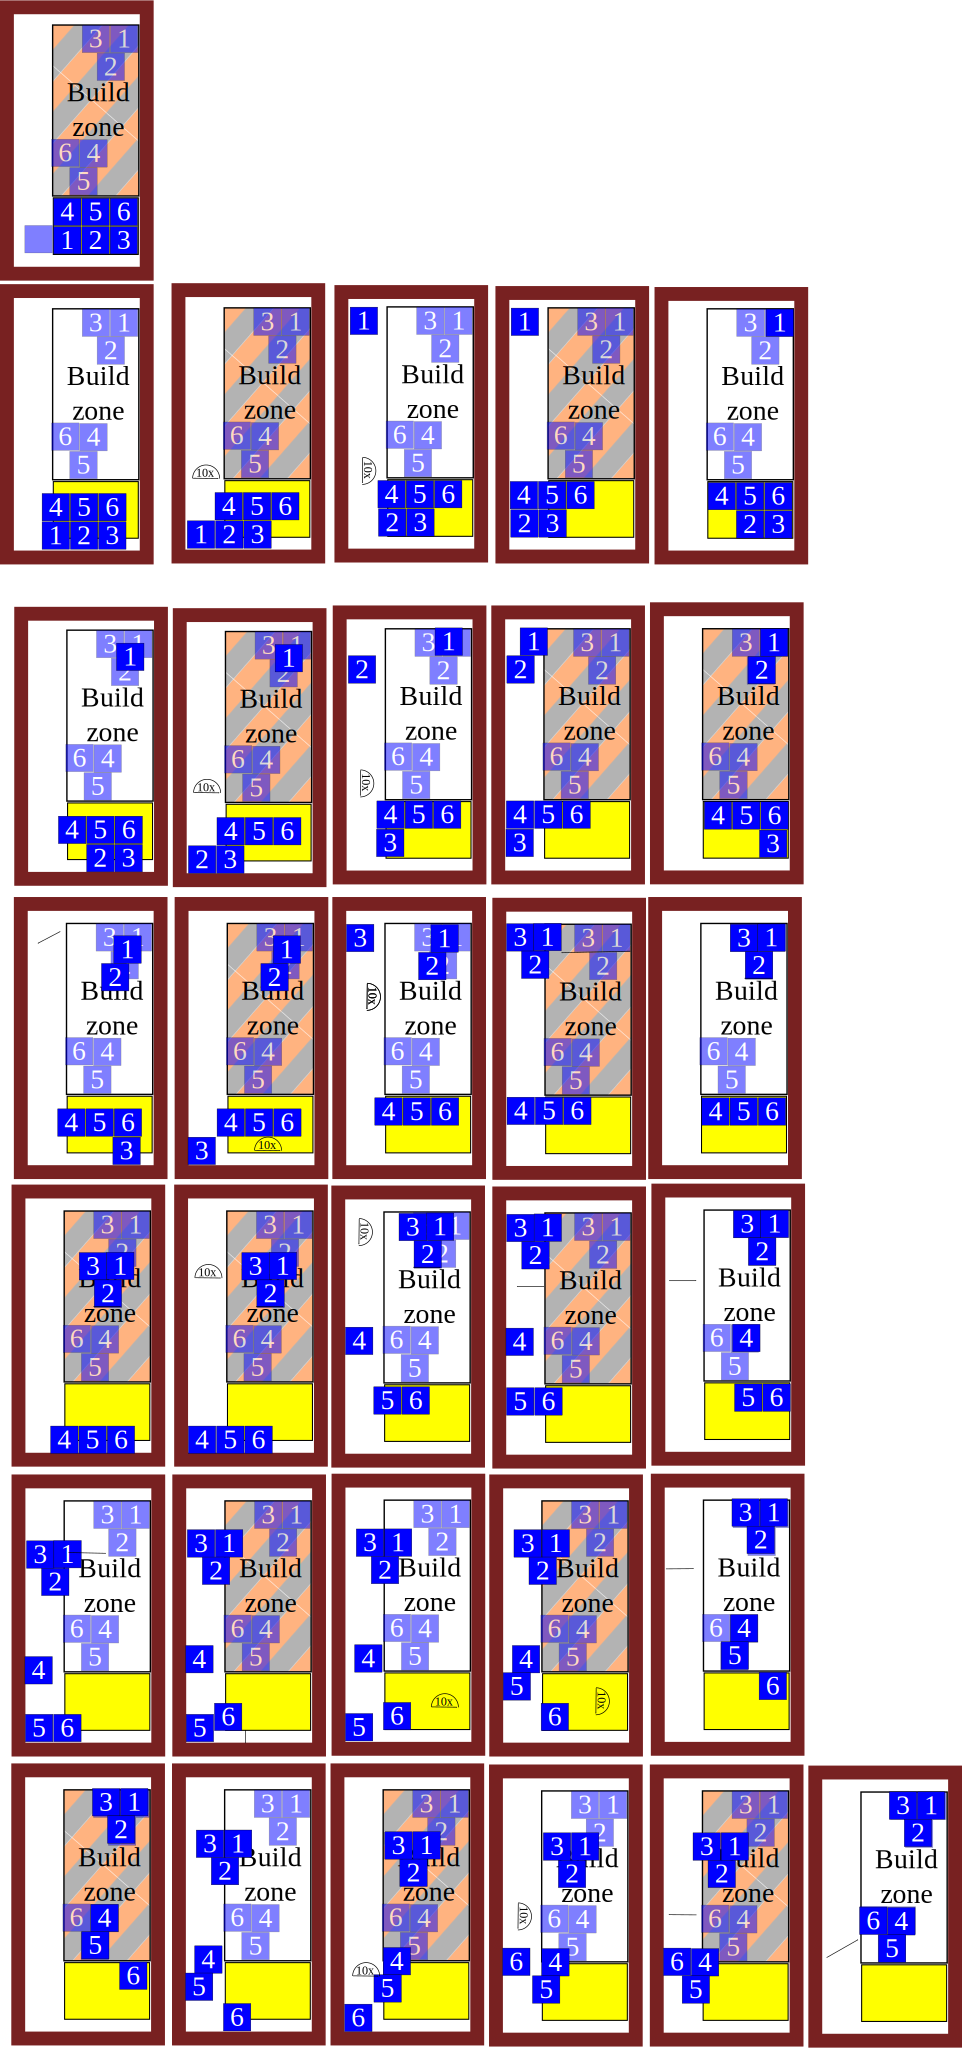
\includegraphics[width=1.0\columnwidth]{construction2dv2.pdf}
\end{center}
\caption{\label{fig:construction2d}
Illustration of algorithm for position control of $n$ robots using wall friction.
}
\end{figure}
=======
%\begin{figure}
%\begin{center}
%	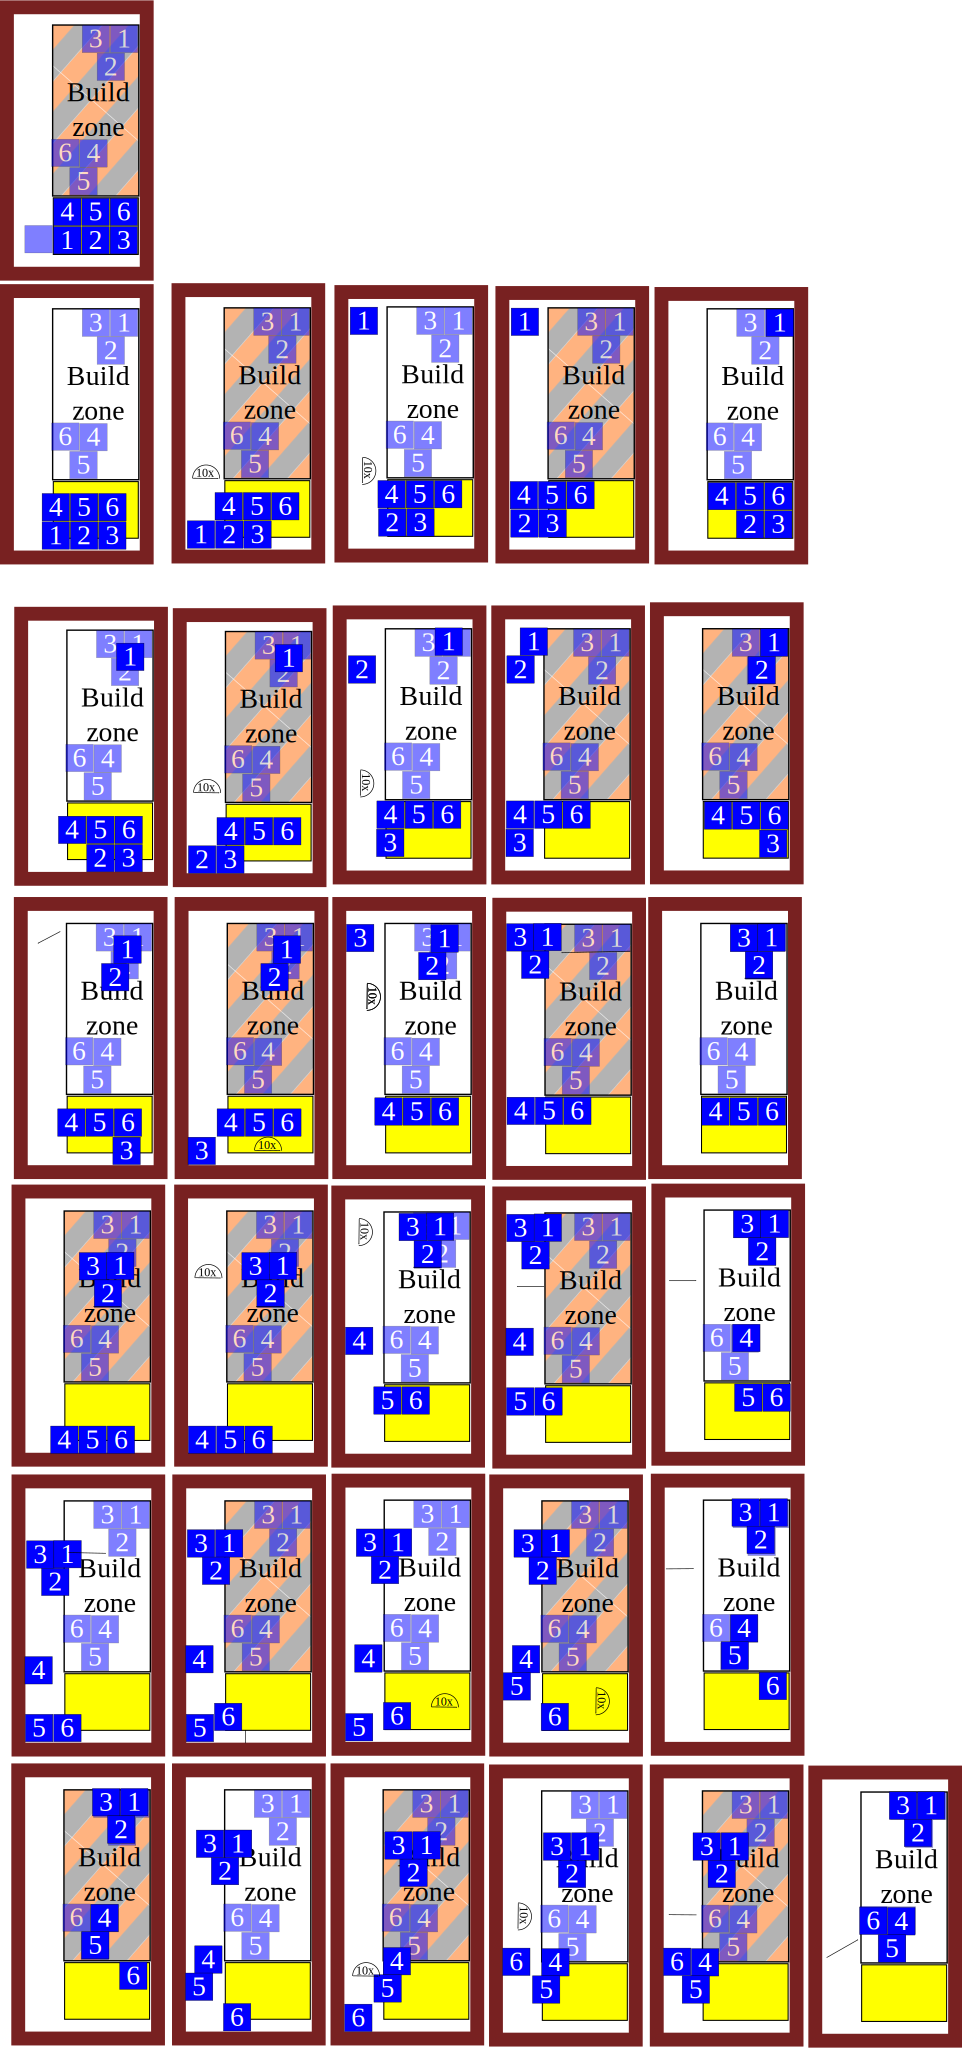
\includegraphics[width=1.0\columnwidth]{construction2dv2.pdf}
%\end{center}
%\caption{\label{fig:construction2d}
%Illustration of algorithm for position control of $n$ robots using wall friction.
%}
%\end{figure}
>>>>>>> Stashed changes




%what images should I show here?
%hysteresis control law, \cite{sadra2014}











%%%%%%%%%%%%%%%
%%%%%%%%%%%%%%%

\section{Simulation}\label{sec:simulation}

Algorithms \ref{alg:PosControl2Robots}, \ref{alg:XControl}, \ref{alg:YControl}, were implemented in Mathematica using point robots (radius = $0$).  All code is available at  a public github repository~\cite{Shahrokhi2015GitHubShapeControl}.  Two trials are shown in Figs. \ref{fig:shapeControlMathematica1} and \ref{fig:shapeControlMathematica2}, showing the initial positions, goal positions, and the path derived by Alg. \ref{alg:PosControl2Robots}.


\textcolor{red}{Shiva:  what is the complexity of this algorithm?  How many steps in the worst case?  When does worst case happen?}





\begin{figure*}
\centering
\renewcommand{\figwid}{0.4\columnwidth}
{\begin{overpic}[width =\figwid]{two_1.png}\put(45,75){$t$  = 0 s}
\end{overpic}
\begin{overpic}[width =\figwid]{two_2.png}\put(45,75){$t$  = 0.25 s}
\end{overpic}
\begin{overpic}[width =\figwid]{two_3.png}\put(45,75){$t$  = 0.5 s}
\end{overpic}
\begin{overpic}[width =\figwid]{two_4.png}\put(45,75){$t$  = 0.75 s}
\end{overpic}
\begin{overpic}[width =\figwid]{two_5.png}\put(45,75){$t$  = 1 s}
\end{overpic}}
\vspace{-1em}
\caption{\label{fig:shapeControlMathematica1}{Frames from an implementation of Alg.\ \ref{alg:PosControl2Robots}: two robot positioning using walls with infinite friction.
Robot initial positions are shown by a crosshair, and final positions by a circled crosshair.  Dashed lines show the shortest route if robots oculd be ocntrolled independently.  The path given by  Alg.\ \ref{alg:PosControl2Robots} is shown with solid arrows.
}
%\vspace{-2em}
}
\end{figure*}

\begin{figure*}
\centering
\renewcommand{\figwid}{0.4\columnwidth}
{\begin{overpic}[width =\figwid]{one_1.png}\put(45,75){$t$ = 0 s}
\end{overpic}
\begin{overpic}[width =\figwid]{one_2.png}\put(45,75){$t$ = 0.25 s}
\end{overpic}
\begin{overpic}[width =\figwid]{one_3.png}\put(45,75){$t$  = 0.5 s}
\end{overpic}
\begin{overpic}[width =\figwid]{one_4.png}\put(45,75){$t$  = 0.75 s}
\end{overpic}
\begin{overpic}[width =\figwid]{one_5.png}\put(45,75){$t$  = 1 s}
\end{overpic}}
\vspace{-1em}
\caption{\label{fig:shapeControlMathematica2}{Two robot positioning: switching positions using walls with infinite friction.  Code available at~\cite{Shahrokhi2015GitHubShapeControl}.}
%\vspace{-2em}
}
\end{figure*}






%%%%%%%%%%%%%%%
%%%%%%%%%%%%%%%

%%%%%%%%%%%%%%%%%%%%%%%%%%%%%%%%%%%%%%%%%%%%%%%%%%%%%%%%%%%
\section{Block-Pushing Results}\label{sec:expResults}
%%%%%%%%%%%%%%%%%%%%%%%%%%%%%%%%%%%%%%%%%%%%%%%%%%%%%%%%%%%

This section analyzes a \emph{block-pushing} task attempted by both our hybrid hysteresis-based controller and by human users.  All experiments used the 2D physics engine box2D~\cite{catto2010box2d}, running in a Chrome web browser on a 2.6 GHz Macbook.  \href{https://github.com/aabecker/SwarmControlSandbox/blob/master/exampleControllers/BlockPushingIROS2015.html}{All code is available at}~\cite{Shahrokhi2015}.
\subsection{Human-Controlled Block-Pushing}

In previous work over 1000 human users completed an online version of this task using varying levels of feedback.
 The original experiment explored manipulation with varying amounts of sensing information: {\bf full-state} sensing showed the position of all robots; {\bf convex-hull} drew a convex hull around the outermost robots; {\bf mean} displayed the average position of the population; and {\bf mean + variance} added a confidence ellipse. Fig.~\ref{fig:Visualization} shows screenshots of the same robot swarm with each type of visual feedback. Full-state requires $2n$ data points for $n$ robots. Convex-hull requires at worst $2n$, but usually a smaller number.  Mean requires two, and variance three, data points.  Mean and mean + variance are convenient even with millions of robots. We hypothesized a steady decay in performance as the amount of visual feedback decreased.

\begin{figure}[b!]
\renewcommand{\figwid}{0.24\columnwidth}
\begin{overpic}[width =\figwid]{VaryVisFS.pdf}\put(20,15){Full-state}\end{overpic}
\begin{overpic}[width =\figwid]{VaryVisCH.pdf}\put(10,15){Convex-hull}\end{overpic}
\begin{overpic}[width =\figwid]{VaryVisMV.pdf}\put(10,15){Mean + var}\end{overpic}
\begin{overpic}[width =\figwid]{VaryVisMe.pdf}\put(30,15){Mean}\end{overpic}
\vspace{-2em}
\caption{\label{fig:Visualization}Screenshots from a block-pushing task with human users. This experiment challenged players to quickly steer 100 robots (blue discs) to push an object (green hexagon) into a goal region. 
%\vspace{-1em}
}
\end{figure}

\begin{figure}
\centering
\begin{overpic}[width = \columnwidth]{ResVaryVis.pdf}\end{overpic}
\vspace{-2em}
\caption{\label{fig:ResVaryVis} Completion-time results for the four levels of visual feedback shown in Fig.~\ref{fig:Visualization}. 
%\vspace{-2em}
}
\end{figure}



To our surprise, the results indicated the opposite: players with just the mean completed the task faster than those with full-state feedback.  As Fig.~\ref{fig:ResVaryVis} shows, the levels of feedback arranged by increasing completion time are [mean, mean + variance, full-state, convex-hull].  Interviews with  beta-testers suggests that tracking 100 robots was overwhelming---similar to schooling phenomenons that confuse predators---while working with just the mean + variance was like using a ``spongy'' manipulator. Convex-hull feedback was confusing and irritating because a single robot left behind an obstacle would distort the entire hull, obscuring the information about the majority of the swarm.
%obscuring what the rest of the swarm is doing.   


\subsection{Automated Block-Pushing}

\begin{algorithm}
\caption{Block-pushing controller for a robotic swarm.}\label{alg:BlockPushing}
\begin{algorithmic}[1]
\Require Knowledge of swarm mean $[\bar{x},\bar{y}]$, the moveable block's center of mass $\mathbf{b}$, a map of the environment, and the locations of all convex corners $\mathbf{C}$
\Require Robot distribution is unimodal
\Require Obstacle-free, straight-line path from swarm to moveable block
\State Compute $\mathbf{M}$, the distance to goal, with breadth-first search
\State Compute the gradient, $\nabla \mathbf{M}$
\State $\mathbf{C} \gets \mathrm{sort(\mathbf{C})}$ according to $-\mathbf{M}$
\While{$\mathbf{b}$ is not in goal region}
\State $\sigma^2 \gets \max{(\sigma_x,\sigma_y)}$
\If {$\sigma^2 > \sigma_{max}^2$}
\While{$\sigma^2 > \sigma_{min}^2$}
\State $\mathbf{c}_i \gets$ the nearest corner in $\mathbf{C}$ to $[\bar{x},\bar{y}]$
\State $ [x_{goal}, y_{goal}] \gets \mathbf{c}_i $
\If {$\mathbf{M}(\mathbf{b}) > \mathbf{M} (\mathbf{c}_i)$}
\State  $[x_{goal}, y_{goal}] \gets  \mathbf{c}_{i-1}$ 
\State Apply \eqref{eq:PDcontrolPosition} to move toward $[x_{goal}, y_{goal}]$
\EndIf
\EndWhile
\Else  
\If {$\mathrm{distance}( \mathbf{b}, [x_{goal}, y_{goal}] ) > 2.5 r_b$}
	\State$r_p \gets 1.5 r_b$  \Comment{guarded move}
	\Else
	\State$r_p \gets 0.1 r_b$  \Comment{pushing move}
	\EndIf
\State $[x_{goal}, y_{goal}] \gets \mathbf{b} - r_p \nabla \mathbf{M}(\mathbf{b})$ 
\EndIf
\State Apply \eqref{eq:PDcontrolPosition} to move toward $[x_{goal}, y_{goal}]$
\EndWhile
\end{algorithmic}
\end{algorithm}



\begin{figure*}
\centering
\renewcommand{\figwid}{0.4\columnwidth}
\begin{overpic}[width =\figwid]{story1.png}\put(6,15){T = 5 s}
\end{overpic}
\begin{overpic}[width =\figwid]{story2.png}\put(6,15){T = 12 s}
\end{overpic}
\begin{overpic}[width =\figwid]{story3.png}\put(6,15){T = 20 s}
\end{overpic}
\begin{overpic}[width =\figwid]{story4.png}\put(6,15){T = 25 s}
\end{overpic}
\begin{overpic}[width =\figwid]{story5.png}\put(6,15){T = 33 s}
\end{overpic}
\vspace{-1em}
\caption{\label{fig:story}Snapshots showing the block-pushing experiment with 200 robots under automatic control.  See the video attachment for an animation. 
%\vspace{-2em}
}
\end{figure*}

\begin{figure}
\centering
\begin{overpic}[scale=0.2]{BFSMode.png}
\end{overpic}
\begin{overpic}[scale=0.2]{GradientView.png}
\end{overpic}
\vspace{-2em}
\caption{\label{fig:BFSGradient}The BFS algorithm finds the shortest path for the moveable block (left), which is used to compute gradient vectors (right).
%\vspace{-2em}
}
\end{figure}

Fig.~\ref{fig:story} shows snapshots during an execution of this algorithm. To solve this block-pushing task, we discretized the environment. On this discretized grid we used breadth-first search to determine $\mathbf{M}$, the shortest distance from any grid cell to the goal, and generated a gradient map $\nabla \mathbf{M}$ toward the goal as shown in Fig.~\ref{fig:BFSGradient}.  The block's center of mass is at $\mathbf{b}$ and has radius $r_b$. The robots were directed to assemble behind the block at  $\mathbf{b} - 1.5 r_b \nabla \mathbf{M}(\mathbf{b})$, then move to  $\mathbf{b} - 0.1 r_b \nabla \mathbf{M}(\mathbf{b})$ to push the block toward the goal location. We use the hybrid hysteresis-based controller in Alg.~\ref{alg:MeanVarianceControl}  to track the desired position, while maintaining sufficient robot density to move a block by switching to minimize variance whenever variance exceeds a set limit. The minimize variance control law \eqref{eq:PDcontrolVariance} is slightly modified to choose the nearest corner further from the goal than $\mathbf{b}$ with an obstacle-free straight-line path to $\mathbf{b}$. 
The control algorithm  for block-pushing is listed in Alg.~\ref{alg:BlockPushing}. 
Experimental results are summarized in Fig.~\ref{fig:AutoControlVaryN}.  Although larger populations of robots can apply more force, minimizing the variance requires more time with larger populations and dominates task completion time.



\begin{figure}
\centering
\begin{overpic}[width = \columnwidth]{AutoControlVaryN.pdf}\end{overpic}
\vspace{-2em}
\caption{\label{fig:AutoControlVaryN} Completion-time results using the automatic controller from Alg.~\ref{alg:BlockPushing} for different numbers of robots.  Each bar is labelled with the number of trials.
}
\end{figure}





Algorithm \ref{alg:BlockPushing} is an imperfect solution and has a failure mode if the robot swarm becomes multi-modal with modes separated by an obstacle, as shown in Fig.~\ref{fig:Failure}.  In this case, moving toward a corner will never reduce the variance below $\sigma_{min}^2$.


  The first challenge is to identify when the distribution has become multi-modal.  Measuring just the mean and variance is insufficient to determine if a distribution is no longer unimodal, but if the swarm is being directed to a corner, and the variance does not reduce below $\sigma_{min}^2$, the swarm has become separated. In this case, we must either manipulate with a partial swarm, or run a gathering algorithm.  For the  `{\sffamily S}'-shaped workspace in this study, an open-loop input that commands the swarm to move in succession \{{\sc left, down, right, down}\} will move the swarm to the bottom right corner.
This is not true for all obstacle fields. In a  `{\sffamily T}'-shaped workspace, it is not possible to find an open-loop input that will move the entire swarm to the bottom of the `{\sffamily T}'.  
 
  Using only the mean and variance may be overly restrictive.  Many heuristics using high-order moments have been developed to test if a distribution is multimodal~\cite{haldane1951simple}.  Often the sensor data itself, though it may not resolve individual robots, will indicate multi-modality.  For instance CCD images reveal clusters of bacteria, and MRI scans show agglomerations of particles~\cite{stuber2007positive}.  This data can be fitted with K-means or expectation maximization algorithms, and manipulation could be performed with the nearest swarm of sufficient size.
  

\begin{figure}
\centering
\begin{overpic}[scale=0.2]{FailureBlockPush.png}
\end{overpic}
\begin{overpic}[scale=0.2]{FailureBlockPushing}
\end{overpic}
\vspace{-1em}\caption{Algorithm \ref{alg:BlockPushing} fails when some robots are separated by the maze and the swarm can not achieve $\sigma^2 < \sigma_{min}^2$.  These failures occured during 14\% of trials.\label{fig:Failure}
%\vspace{-2em}
}
\end{figure}








%%%%%%%%%%%%%%%
%%%%%%%%%%%%%%%
%%%%%%%%%%%%%%%%%%%%%%%%%%%%%%%%%%%%%%%%%%%%%%%%%%%%%%%%%%%
\section{Conclusion and Future Work}\label{sec:conclusion}
%%%%%%%%%%%%%%%%%%%%%%%%%%%%%%%%%%%%%%%%%%%%%%%%%%%%%%%%%%%


This paper presented techniques for controlling the orientation of an object by manipulating it using a swarm of simple robots with global inputs.
The paper provided algorithms for precise orientation control, as well as demonstrations of orientation control. 


Future efforts should be directed toward optimizing torque control, applying the techniques to hardware robots, pose control for multiple part assembly, and manipulation in a crowded workspace.
The control laws in this paper used only the mean and variance of the swarm.  The control techniques may be optimized using high-order moments, or by stochastic modeling of the collisions between swarm members and the object.

%TODO JOURNAL: design controllers that efficiently regulate $\sigma_{xy}$.
%TODO JOURNAL: We will design Lyapunov-inspired controllers for $\sigma_{xy}$ to prove controllability. 
%TODO JOURNAL:  and rank controllability as a function of friction.
% TODO: JOURNAL: and vary wall friction by laser-cutting boundary walls with a variety of profiles. 


%    Inspired by large-scale human experiments with swarms of robots under global control,  this paper investigated controllers that use only the mean and variance of a robot swarm. We proved that the mean position is controllable, and provided conditions under which variance is controllable.  We derived automatic controllers for each and a hysteresis-based switching control that controls the mean and variance of a robot swarm.  We employed these controllers as primitives for a block-pushing task. 
%    
%    Future work should implement these controllers on a robot swarm and decrease completion time by avoiding counter-productive contact with the block while the swarm is lowering its variance.  We have also assumed the swarm is unimodal and has a straight-line path to the moveable block. Relaxing these assumptions requires solving the \emph{gathering problem}.  The gathering problem for a swarm with uniform inputs is largely unexplored, and must be examined probabilistically for nontrivial environments.
%    
    % We should also control the covariance $\sigma_xy$ and higher moments of the distribution
    
    
    
%Sensing is expensive, especially on the nanoscale. To see nanocars~\cite{Chiang2011}, scientists fasten molecules that fluoresce light when activated by a strong light source. Unfortunately, multiple exposures can destroy these molecules, a process called \emph{photobleaching}. Photobleaching can be minimized by lowering the excitation light intensity, but this increases the probability of missed detections~\cite{Cazes2001}. A control methodology based on statistics of the robot swarm rather than the actual position of each robot, allows relaxing demands on imagine systems, controllers robust to tracking errors, and a simpler methodology.  In this work we...
%


% Additionally, as population characteristics, they are available even if only a percentage of the robots are detected each control cycle.
%Photobleaching: http://www.piercenet.com/browse.cfm?fldID=4DD9D52E-5056-8A76-4E6E-E217FAD0D86B
%
%Photobleaching is caused by the irreversible destruction of fluorophores due to either the prolonged exposure to the excitation source or exposure to high-intensity excitation light. Photobleaching can be minimized or avoided by exposing the fluor(s) to the lowest possible level of excitation light intensity for the shortest length of time that still yields the best signal detection; this requires optimization of the detection method using high sensitivity CCD cameras, high numerical aperture objective and/or the widest bandpass emission filter(s) available. Other approaches include using fluorophores that are more photostable than traditional fluorophores and/or using antifade reagents to protect the fluor(s) against photobleaching. Steps to avoid photobleaching are not feasible for all detection methods and should be optimized for each method used. For example, antifade reagents are toxic to live cells, and therefore they can only be used with fixed cells or tissue. Furthermore, some detection methods, such as flow cytometry, normally do not require steps to avoid photobleaching because of the extremely short exposure time of the fluorophore to the excitation source.
%%%%%%%%%%%%%%%



%\missingfigure[figwidth=6cm]{Intro: image of real kilobots making torque to a rectangular object}
%\missingfigure[figwidth=6cm]{Theory: drawing of an object that illustrates what torque and force is}
%\missingfigure[figwidth=6cm]{Simulation: snapshots of the simulation doing torque control with blue disks}
%\missingfigure[figwidth=6cm]{Simulation: plot showing angular velocity of the object and the goal angles}
%\missingfigure[figwidth=6cm]{Experiment:plot showing angular velocity of the object and the goal angles }
%\missingfigure[figwidth=6cm]{Experiment: snapshots of the kilobots doing torque control of a rectangular object}



    
\section{Acknowledgements}
%RULES: http://www.nsf.gov/pubs/policydocs/pappguide/nsf16001/aag_6.jsp
This material is based upon work supported by the National Science Foundation under Grant No.\ 
\href{http://nsf.gov/awardsearch/showAward?AWD_ID=1553063}{ IIS-1553063}.
%Optional disclaimer (mandatory for non-scientific)
Any opinions, findings, and conclusions or recommendations expressed in this material are those of the authors and do not necessarily reflect the views of the National Science Foundation.
%We acknowledge many \href{http://mrsl.rice.edu/}{mrsl.rice.edu} lab members who helped beta test \href{http://www.swarmcontrol.net}{SwarmControl.net}; helpful discussion with \href{http://www.jmtour.com/}{James Tour}, \href{http://slink.rice.edu/}{Stephan Link}, and Victor Garc\`ia L\`opez on fabrication and visualization challenges at the nanoscale with nanocars; and the \href{http://cttl.rice.edu/}{Rice Center for Technology in Teaching and Learning}.
%This work was partially supported by the National Science Foundation under 
%\href{http://www.nsf.gov/awardsearch/showAward?AWD_ID=1035716}{CPS-1035716}.  
   
\bibliographystyle{IEEEtran}
\bibliography{IEEEabrv,TorqueControl,../../../RoboticSwarmControlLab/bib/aaronrefs}
\end{document}


%/Users/ab55/Desktop/svn/MRSL-Papers/Drafts-Current/2013-03-13-IROS-MassiveUniformManipulation/document
%/Users/ab55/Desktop/svn/ensemble/bib





